  \subsection{Figura de Lissajous}
               
      Las figuras de Lissajous son comúnmente usadas para la determinación de la diferencia
      de fase entre dos señales de la misma frecuencia. Los osciloscopios cuentan con un modo
      conocido como \textbf{modo X-Y}, el cual toma una de las señales y la inyecta en el canal
      1, y la otra en el canal 2, de esa manera, internamente el osciloscopio se encarga de 
      usar estas señales para los trazos horizontal y vertical, y así se forma la figura de
      Lissajous. 

         \begin{figure}[H]
            \centering
            \frame{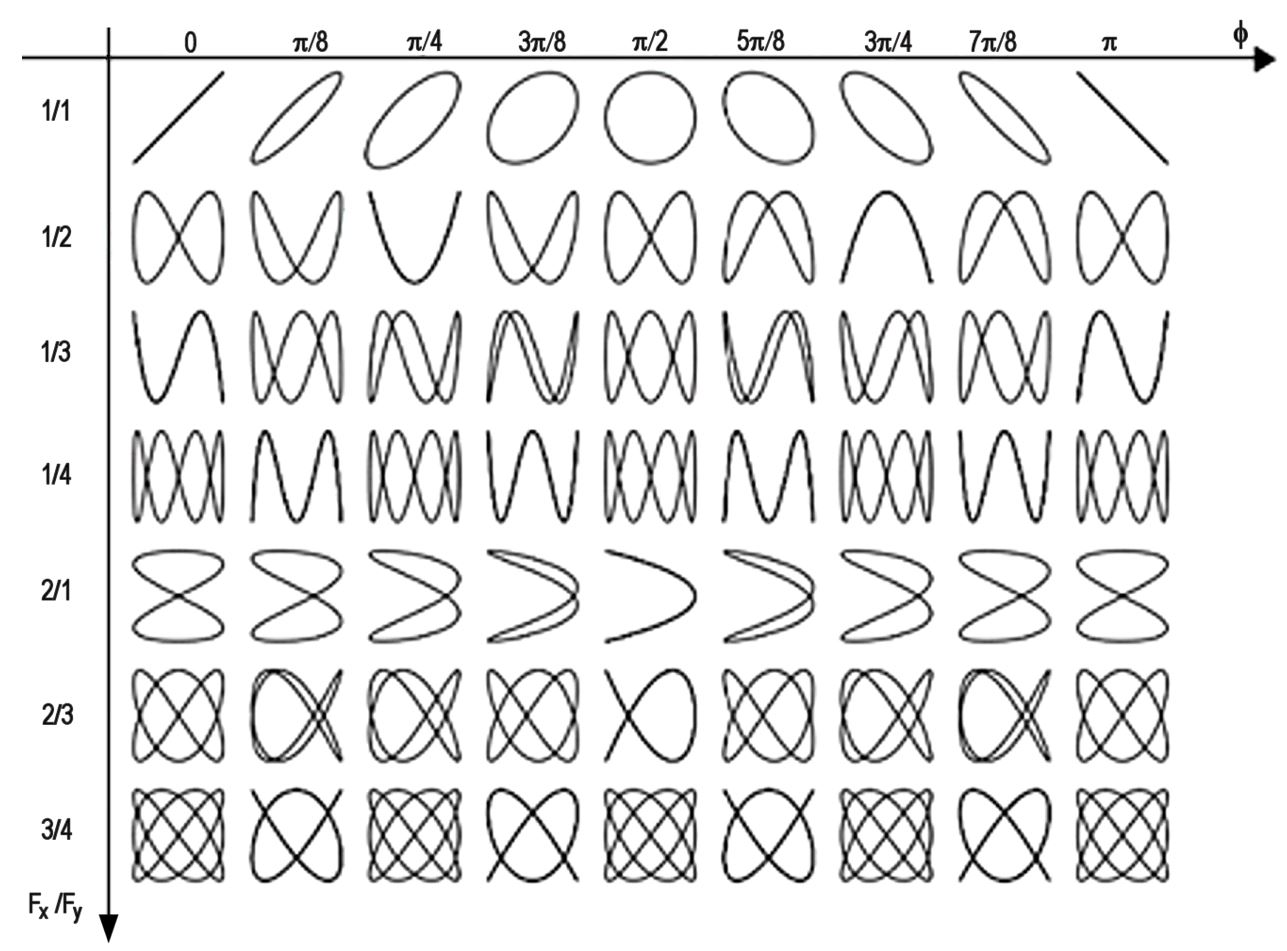
\includegraphics[width=.7 \textwidth]{Imagenes/MarcoTeorico/LissajousFiguras.jpg}}
            \caption{Figuras de Lissajous.}
            \label{fig:LissajTipos}                 
         \end{figure}

      De los tipos de curvas de Lissajous vistas en la Figura \ref{fig:LissajTipos}, 
      en el presente trabajo práctico, se destacará la figura de tipo \textbf{elíptica}, 
      las cuales son formadas por señales con valores de fase distintos a $\dfrac{\pi}{2}$ 
      y/o con diferentes amplitudes.

      \begin{figure}[H]
         \centering
         \frame{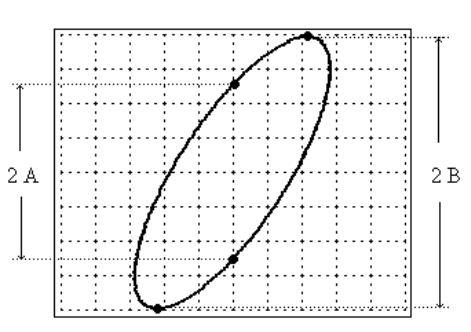
\includegraphics[width=.5 \textwidth]{Imagenes/MarcoTeorico/LissajousEliptico.png}}
         \caption{Figura de Lissajous de tipo elíptico.}
         \label{fig:LissajElip}           
      \end{figure}
      
      \newpage
      La obtención de la diferencia de fase entre las señales se pueden determinar de la
      siguiente manera.
      Considerando las siguientes expresiones
      \begin{align}
         x &= X\cdot \sin(\omega t) \hspace{10pt} ; \hspace{10pt} y = B\cdot \sin(\omega t + \varphi) \ , \notag
      \end{align}
      
      \noindent de la Figura \ref{fig:LissajElip}, para $x = 0$ se deduce que
      \begin{align}
         x &= X\cdot \sin(\omega t) = 0 \hspace{10pt} \Longrightarrow \hspace{10pt} t = 0 ~ , \notag \\
         \intertext{por lo tanto}
         y &= B\cdot \sin(\omega 0 + \varphi) = B\cdot \sin(\varphi) = A ~ . \notag 
      \end{align}   

      \noindent Finalmente
      \begin{align}
         \sin(\varphi) = \dfrac{A}{B} ~ . \notag
      \end{align}
      
      \noindent De la última ecuación se despeja el ángulo de desfase
      \begin{equation}
         \boxed{\varphi = \sin^{-1}\ \left(\dfrac{A}{B} \right)}   \ . \label{eqn:AngDeDesf}   
      \end{equation}

